\documentclass[a4paper]{article}

\usepackage{graphicx}
\usepackage{amsmath}
\usepackage{hyperref}

\usepackage[utf8]{inputenc}
\usepackage[margin=0.5in]{geometry}

\title{Discrete choice and pseudo-random errors in MATSim}
\author{Sebastian Hörl}
\date{April 2020}

\begin{document}

\maketitle

\section*{Repository}

\begin{itemize}
  \item Code is at \url{https://github.com/sebhoerl/matsim-pseudo-random-errors}
  \item Latex is at \texttt{/latex}
  \item Notebook for running + plots is at \texttt{Analysis.ipynb}
\end{itemize}

\section{Introduction}

\begin{itemize}
    \item Currently, no taste variation in MATSim
    \item MATSim based on utility maximization
    \item Aim 1: Explain in detail how choice process in MATSim works and how it is different from discrete choice models
    \item Aim 2: Present a way to bring DCM and MATSim closer to each other with pseudo-random errors terms
\end{itemize}

\section{MATSim choice process}

Toy example:

\begin{itemize}
    \item Point X and Point Y
    \item $N$ agents with a plan that consists of an activity at $X$ and an activity at $Y$, connected by a trip
    \item The trip can either by mode $A$ (e.g. car) or mode $B$ (e.g. pt)
    \item Initially, the trip is teleported with the same speed and distance factor, i.e. the two options are equal.
    We start with 100\% of the trips with mode $A$
    \item The simulation uses a selection startegy (BestScore or ChangeExpBeta) and an innovation strategy (ChangeLegMode)
    \item Each experiment we run 20 times with different random seeds.
\end{itemize}

\begin{figure}[h!]
    \centering
    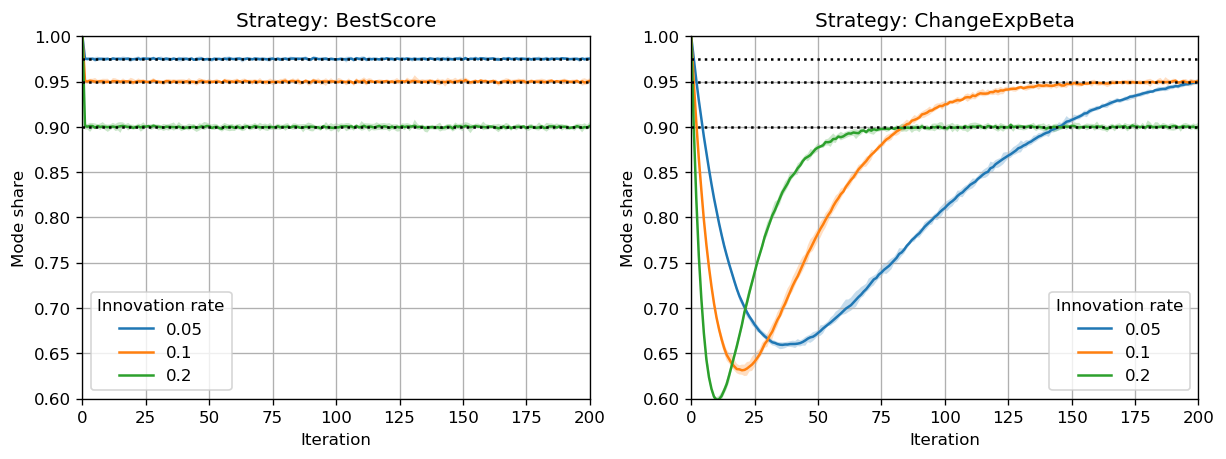
\includegraphics[width=\textwidth]{images/standard_behaviour.png}
    \caption{Standard behaviour}
    \label{fig:standard_behaviour}
\end{figure}

\begin{itemize}
  \item We start with a per-trip scoring. A $A$ trip gives a score of $-1.0$, a $B$ trip gives a score
  of $-2.0$.
  \item Figure \ref{fig:standard_behaviour} shows the standard MATSim behaviour with two different
  replannign strategies (BestScore and ChangeExpBeta) for different innovation rates. They show
  the mode share of mode $A$. First, it starts with 100\%, then it goes down and for the ChangeExpBeta
  we make jumps back (in the agent memory of three plans). Eventually, we stabilize over the
  iterations at a mode share that represents the replanning rate.
  \item Because the score of $A$ is better, the agents select usually this mode. Only in the case when
  they do a ChangeLegMode $B$ is chosen, so the share of $B$ equals $\frac{1}{2} \rho$ with $\rho$ being the
  replanning rate.
  \item NOTE: The ChangeLegMode strategy was modified here, because in the current MATSim version it only
  proposes modes, which are NOT currently chosen. In that case innovation from A would always lead to
  B and the other way round. In essence, one then has a mode share of exactly $\rho$ for B.
\end{itemize}

\begin{figure}[h!]
    \centering
    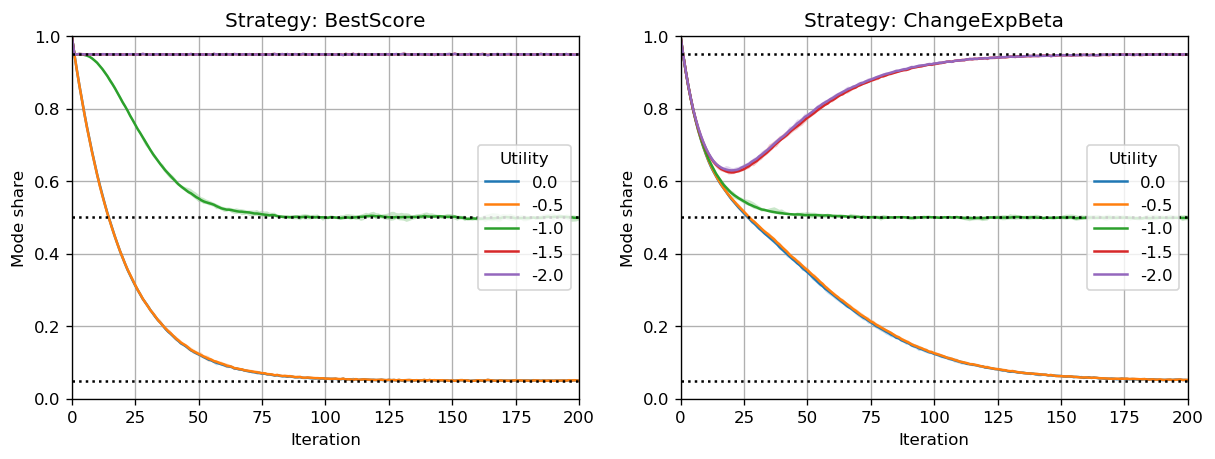
\includegraphics[width=\textwidth]{images/vary_scores.png}
    \caption{Varying scores with utility maximization}
    \label{fig:vary_scores}
\end{figure}

\begin{itemize}
  \item In Figure \ref{fig:vary_scores} the experiment is repeated with an
  innovation rate of 10\%. Clearly, the mode share goes again
  to 95\%, but here we vary the scores. One mode has a score of $-1.0$ here
  while the score for the other mode is varied. The plot shows nicely that
  the magnitude of the value does not matter when looking where the system
  converges, the only thing that matters is which mode is the better
  one.
  \item The experiment could probably be improved by choosing lower
  magnitudes in general, I suppose that then we would see a difference in
  convergence speed for ChangeExpBeta.
  \item In any case, the experiment shows the big difference to choice models.
  A choice modeller working with MATSim who sees the parameters (which are not
  called utility parameters, but scoreing parameters, to be fair!) would
  probably expect that changing these values would substantially influence
  the mode share. Clarifying this is one aim of this paper.
  \item But this also shows that one can not easily port utility parameters
  from a discrete choice model to MATSim, because the magnitude of the values
  does not vary.
\end{itemize}

This would be the point here to discuss constrained cases. One may see more
diverse mode choices when parameters from a discrete choice model are applied,
but they would stem from constraints that are built into the simulation.
Most importantly, agents who have generally better parameters for car would
potentially not use the car, because of congestion and select another
mode of transport. It would then be interesting discuss how those constriants
translate to the discrete choice model.

From our analyses with a pure DMC implementation in MATSim we saw that we can
usually take trip-based discrete choice models and they would produce a good
fit with reference mode shares if (and only if) we add sensible constraints
such as vehicle continuity.

\section{Adding pseudo-random errors}

\begin{itemize}
  \item MNL models (and other close form choice models) are baesd on formulations
  somewhat like $k^* = \text{arg max}_k \{ u_1, ..., u_k, ... \}$ between
  different alternatives with different utilities. The utilities would then be
  separable into a deterministic part and a random part as  $u_k = v_k + \sigma \epsilon$.
  Clearly, here the variability in choice (and taste) is directly included in
  the model.
  \item When we look at mode shares, we are interested in the population-wide
  mode shares, so we look at a share over all persons. We can then assume that
  the errors for one combination of person, trip and mode are always the
  same, i.e. they are following a certian distribution if looked at from above
  over the whole population, but they are fixed on the individual level.
  \item Above we have established that MATSim tries to maximize the score
  of the agents plans. In the DCM one wants to find the maximum utility
  alternative, given the deterministic and random part. So MATSim basically
  already provided all that is necessary to perofrm the optimization part, it
  is only missing the error terms to exactly replicate a DCM.
\end{itemize}

\subsection{Cryptographic hash functions}

\begin{itemize}
  \item In cryptography, hash functions $O = H(I)$ are used which get a variable length series
  of bits as input and return a fixed-size series of bits as output. The idea is
  that whenever the same input $I$ is provided, the same output $O$ is generated.
  At the same time, the input $I$ should not be possible to reconstruct from the
  output $O$. This way, websites would ``hash'' the password of their users and
  only save the output $O$ in their database. It would then not be possible to
  reconstruct the password, but when the user provides the password again
  to log in, it can be tested whether he or she entered the correct password
  by hashing it again and comparing the two hashes.
  \item Many cryptographic hash functions (like SHA-256) are constructed around
  the ``avalanche effect'' which says that if only one bit in the input changes,
  more than 50\% of the output bits should change. Given a ground set of inputs
  $I_1, ..., I_N$ this means that the hashes in their output domain (for
  4 bit hashes this would be $0000$ to $1111$) are uniformly distributed.
  \item Hence, given a combination of values, we can hash them and obtain
  uniformly distributed random variables.
\end{itemize}

\subsection{Application to MATSim}

\begin{itemize}
  \item We can define an input string $I = (Preson Id, Trip Index, Mode)$
  and convert it to a byte array in Java. Java also readily provides cryptographic
  hashing functions, here we use SHA-256. Given the output $O$ we can divide
  the output by the maximum number of its output domain of 256 bit (which is not
  completely straightforward as a normal \texttt{long} in Java only has 64bit).
  \item All that remains then is to add an additional component to the
  \texttt{SumScoringFunction} of MATSim and add an error to the score of an
  ongoing plan whenever a trip is performed.
  \item Here, we obtain a uniformly distributed sample $u$ through the hashing
  function and then transform it to a Gumbel-distributed variable through
  linear transformation.
  \item Figure \ref{fig:errors} shows the simulation outcome. Again, for one
  mode the (deterministic) score per trip is varied. Clearly, we now repliate
  the mode shares that a discrete choice model like $P(k) = \exp(-beta_k) / \left( \exp(-beta_A) + \exp(-beta_B) \right)$ would produce.
  \item This is a sensible way of integrating parameters from a discrete choice
  model into MATSim.
  \item HOWEVER: Note that the reference values (shown as dashed lines) in
  Figure \ref{fig:errors} are corrected from the discrete choice model. Given
  the share for mode $A$ from the model as $P_A$ it is altered through the
  innovation process of MATSim. In fact, the mode shares in the simulation do
  not show $P_A$, but $P_A \cdot \rho + \frac{1}{2} \rho$. Nevertheless, we
  can this way establish a connection between the theory and practice of
  discrete choice models and MATSim.
  \item The influence of the innovation rate is also shown in Figure \ref{fig:replanning_rates}.
  Here, one mode has score $-1.0$ while the other has score $-2.0$. Clearly,
  with a very high replaning rate of 50\% the expected share is strongly
  modified by MATSim, but the resulting value can be predicted analytically.
\end{itemize}

\begin{figure}[h!]
    \centering
    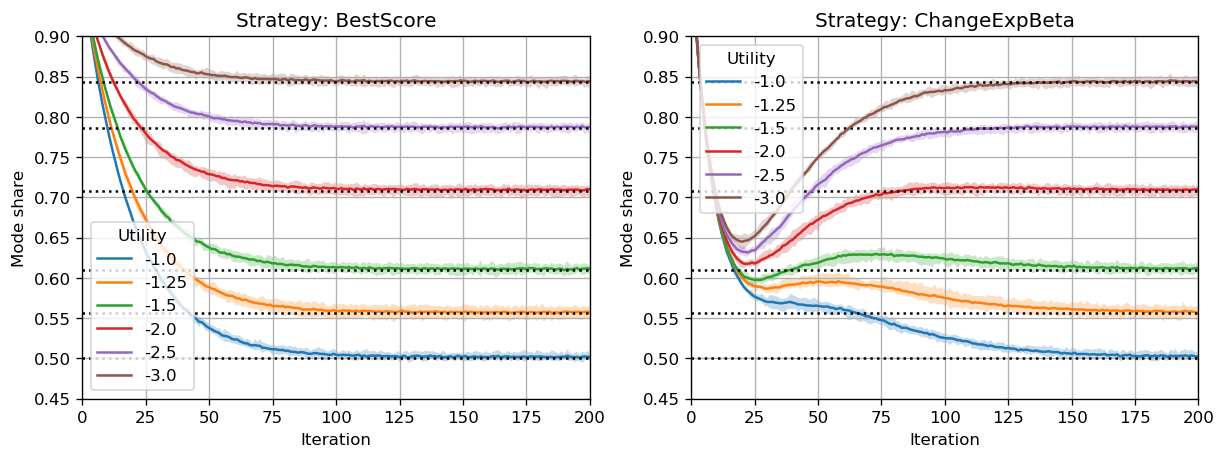
\includegraphics[width=\textwidth]{images/errors.png}
    \caption{Pseudo-random errors}
    \label{fig:errors}
\end{figure}

\begin{figure}[h!]
    \centering
    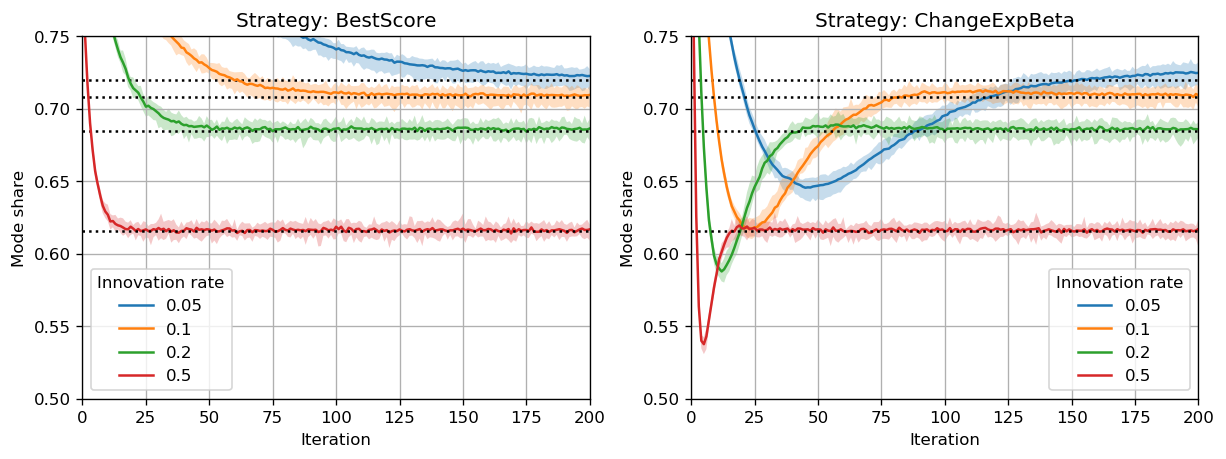
\includegraphics[width=\textwidth]{images/replanning_rates.png}
    \caption{Different replanning rates for pseudo-random errors}
    \label{fig:replanning_rates}
\end{figure}

\section{To be continued ...}

\begin{itemize}
  \item Repeat the experiments in a constrained case (i.e. road capacity for one of the modes)
  \item Explore relationship between choice models and constraints in MATSim
  \item Generalize to departure time choice / location choice / route choice
  \item What about the individual level? We may have cases where an agent has no
  access to public transport or a bike, but randomly the error for the car mode
  is strongly negative. We would then produce plans with unrealistically long
  walk modes. Is this a relevant problem? Can we quantify the probability of
  this happening?
  \item Interestingly, we can also analytically investigate the ``scoring''
  plot of MATSim. Because now we generate EV-distributed scores, of which we
  show the average or the maximum in the the ``scorestats.txt'' plot. For these
  simple examples, we can actually analytically derive these values (especially
  the maximum as Gumbel is maximum-stable). Would be another interesting aspect
  to add to the initial toy example.
  \item Explore the runtime of this in a larger scenario, and also convergence.
  I would assume that the hashing would not substantially slow down the simulation,
  but it would be noticeable. Would we see faster convergence?
  \item ... certainly if we use BestScore, so comparing BestScore with ChangeExpBeta
  in this case is interesting. This especially becomes interesting in the
  constrained case (for the unconstrained case there is no reason \textit{not}
  to use BestScore). Maybe one could think about a combination of BestScore
  and ChangeExpBeta.
  \item All of this could be very interesting in combination with Gunnar's
  approach of making a emulation of the simulation to apply the replanning
  strategies multiple times.
\end{itemize}

\end{document}
